\section{Vererbung}
	Vererbung (englisch inheritance) ist ein Konzept der objektorientierten Programmierung, das meist in Kombination mit
	Polymorphie eingesetzt wird (siehe 3.2.1.2 Vererbungspolymorphie), aber auch eigenständig sinnvoll verwendet werden kann.
	Wenn z.B. Klasse B von Klasse A erbt, werden alle Eigenschaften und Methoden der Basisklasse A (auch Ober-, Super- oder
	Elternklasse) in die abgeleitete Klasse B (auch Unter-, Sub- oder Kindklasse) übernommen. Dies hat den Vorteil, dass
	Eigenschaften und Methoden aus einer bestehenden Basisklasse wiederverwendet werden können, und somit doppelter Code und
	Schreibarbeit vermieden werden. In UML (Unified Modeling Language) wird Vererbung durch einen Pfeil von einer abgeleiteten
	Klasse zu dessen Basisklasse dargestellt.
	
	\begin{figure}[h]
		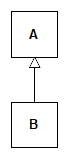
\includegraphics[scale=0.75]{vererbung/uml.png}
	\end{figure}
	
	\subsection{Datenkapselung im Rahmen der Vererbung}
		
		\subsubsection{Änderung der Sichtbarkeit von Eigenschafen und Methoden bei der Vererbung}
			
			Wenn eine Klasse von einer anderen erbt, kann sich die Sichtbarkeit der vererbten Eigenschafen und Methoden ändern.
			
			\begin{table}[H]
	\begin{tabularx}{\textwidth}{$l|^X|^X|^X}
		\multicolumn{4}{l}{\bfseries Sichtbarkeit in ...} \\
		\hline
		\bfseries Basisklasse    & \multicolumn{3}{l}{\bfseries abgeleiteter Klasse (erbt ... von Basisklasse)} \\
		\rowstyle{\bfseries}     & öffentlich    & geschützt                   & privat                      \\
		                         & (``ist-ein'') & (``ist-implementiert-mit'') & (``ist-implementiert-mit'') \\
		\hline
		öffentlich $\rightarrow$ & öffentlich    & geschützt                   & privat                      \\
		geschützt  $\rightarrow$ & geschützt     & geschützt                   & privat                      \\
		privat     $\rightarrow$ & nicht vererbt & nicht vererbt               & nicht vererbt               \\
	\end{tabularx}
\end{table}

			
			Es gibt 3 Arten der Vererbung: die öffentliche, die geschützte und die private Vererbung.
			
			Bei der öffentlichen Vererbung bleiben geschützte Eigenschafen und Methoden der Basisklasse auch in der
			abgeleiteten Klasse geschützt. Öffentliche Eigenschafen und Methoden bleiben öffentlich. Öffentliche Vererbung
			sollte immer eine ``ist-ein''-Beziehung darstellen. Jedoch sollte nicht jede ``ist-ein''-Beziehung durch Vererbung
			dargestellt werden. (siehe ?.?... Kreis-Ellipse-Problem) Diese Art der Vererbung wir am häufigsten verwendet.
			
			Bei der geschützten Vererbung sind alle öffenlichen und geschützten Eigenschafen und Methoden der Basisklasse in
			der abgeleiteten Klasse geschützt. Geschützte Vererbung sollte immer eine ``ist implementiert mit''-Beziehung darstellen
			
			Bei der privaten Vererbung sind alle öffentlichen und privaten Eigenschafen und Methoden der Basisklasse in der
			abgeleiteten Klasse privat.
			Private Vererbung solle wie geschützte Vererbung immer eine ``ist implementiert mit''-Beziehung darstellen.
			Eine gute Alternative zur geschützten und privaten Vererbung bietet das Layering (auch Komposition genannt). Beim
			Layering wird statt von einer Klasse zu erben, eine Eigenschaft
			der Klasse hinzugefügt. Layering stellt eine ``hat-ein''- und somit auch eine ``ist-implementiert-mit''-Beziehung dar.
			
			Private Eingenschafen und Methoden der Basisklasse werden nicht in die abgeleitete Klasse vererbt.
			
			{\bfseries Beispiel:}
		
			\UseRawInputEncoding{\lstinputlisting[language={C++}]{vererbung/beispiele/point/src/point2d.hpp}}\inputencoding{utf8}
			Eine C++ Klasse Point2d, deren Objekte Punkte auf einer Ebene darstellen, existiert bereits. Nun sollen auch Punkte im Raum
			erstellt werden können. Dafür wird die Klasse Point3d geschrieben, welche unterschiedlich programmiert werden kann.
			
			{\bfseries Lösung ohne Vererbung:}
			\UseRawInputEncoding{\lstinputlisting[language={C++}]{vererbung/beispiele/point/src/point3d.no.hpp}}\inputencoding{utf8}
			Diese Lösung ist nicht optimal, da die Eingenschaften x und y aus der Klasse Point2d nicht wiederverwendet werden.
			
			{\bfseries Lösung mit öffentlicher Vererbung:}
			\UseRawInputEncoding{\lstinputlisting[language={C++}]{vererbung/beispiele/point/src/point3d.public.hpp}}\inputencoding{utf8}
			Obwohl hier öffenliche Vererbung verwendet wurde, ist es wahrscheinlich nicht sinnvoll diese Klassen vielgestaltig zu verwenden, da die
			Aussage ``Ein Punkt im Raum (Point3d) ist ein Punkt auf einer Ebene (Point2d).'' nicht stimmt.
			
			\UseRawInputEncoding{\lstinputlisting[language={C++}]{vererbung/beispiele/point/src/point.use.cpp}}\inputencoding{utf8}
			Diese Zeile würde zwar vom Compiler übersetzt werden, macht aber wenig Sinn. Leider gibt es keine Möglichkeit eine
			solche Verwendung zu verhindern. Deshalb ist auch die Lösung mit öffentlicher Vererbung nicht optimal.
			
			{\bfseries Lösung mit privater Vererbung:}
			\UseRawInputEncoding{\lstinputlisting[language={C++}]{vererbung/beispiele/point/src/point3d.private.hpp}}\inputencoding{utf8}
			Wenn man von der Klasse 'Point2d' privat erbt, hat man keines der Probleme der anderen beiden Lösungen,
			allerdings muss man die Eigenschaften x und y in der abgeleiteten Klasse wieder öffentlich machen, da diese bei
			der privaten Vererbung privat werden. In diesem Fall hat diese Lösung keinen Vorteil im Vergleich zur ersten, da
			der Code sogar länger ist. Wenn aber x und y Methoden statt Eigenschaften sind, lohnt es sich sehr wohl private
			Vererbung zu verwenden, da diese dann nicht doppelt implementiert werden müssen.
			
	
	\subsection{Schnittstellenvererbung}
		Bei der Schnittstellenvererbung wird nur die Signatur, aber keine Standardimplementierung, einer Methode der
		Basisklasse	in die abgeleitete Klasse übernommen. Deshalb MÜSSEN alle Methoden, die mittels Schnittstellenvererbung
		vererbt werden, in der abgeleiteten Klasse implementiert werden. In Java ist das Typensystem zweigeteilt, in normale
		Klassen und Interfaces, die von Klassen implementiert werden können. In C++ können Interfaces mit abstrakten Klassen,
		die nur öffentliche virtuelle Methoden enthalten, nachgebildet werden.
		
	\subsection{Implementierungsvererbung}
		Bei der Implementierungsvererbung wird im Gegensatz zur Schnittstellenvererbung nicht nur die Signatur, sondern auch
		die Implementierung einer Methode in die abgeleitete Klasse übernommen. So kann beispielsweise von der Basisklasse ein
		Standardverhalten vorgeschlagen werden, welches aber, falls Notwendig, von der abgeleiteten Klasse überschrieben werden
		kann.
		
	\subsection{Mehrfachvererbung}
		Wenn eine Unterklasse von mehr als einer Oberklasse erbt spricht man von Mehrfachvererbung. Mehrfachvererbung wird
		verwendet, um Features mehrerer Klassen in einer Klasse zu vereinen. Mehrfachinterfacevererbung ist in den meisten
		Fällen problemlos möglich. Mehrfachimplementierungsvererbung jedoch lassen viele Sprachen nicht zu, da diese oft zu 
		fehleranfälligem und unübersichtlichem Code führt. Ein weiteres Problem der Mehrfachimplementierungsvererbung ist, dass
		sich Implementierungen aus unterschiedlichen Basisklassen, widersprechen können.
		\begin{figure}[H]
			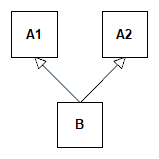
\includegraphics[scale=0.75]{vererbung/mehrfach/mehrfach.png}
		\end{figure}
		
		\subsubsection{Diamond-Problem}
			Das Diamond-Problem ist eines der Probleme, zu denen Mehrfachvererbung führen kann. Dieses tritt auf,
			wenn eine abgeleitete Klasse C über mehr als einen Pfad von derselben Basisklasse A erbt. Dies ist
			problematisch, da die Eigenschaften und Methoden aus Klasse C mehrfach an Klasse A vererbt werden,
			und deshalb in der abgeleiteten Klasse A öfter existieren.
			\begin{figure}[H]
				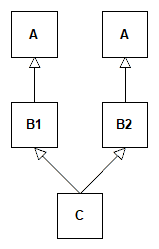
\includegraphics[scale=0.75]{vererbung/mehrfach/diamond/nicht_virtuell.png}
			\end{figure}
			
			\paragraph{C++-Lösung: Virtuelle Vererbung}\mbox{}\\
				In C++ kann das Problem mithilfe virtueller Vererbung gelöst werden. Hierbei wird von allen Klassen, die über
				mehrere Pfade von einer abgeleiteten Klasse beerbt werden, virtuell geerbt. Somit teilen sich dessen
				abgeleitete Klassen eine gemeinsame Instanz von dieser Klasse.
				\begin{figure}[H]
					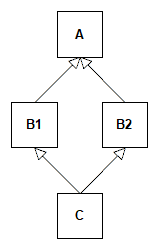
\includegraphics[scale=0.75]{vererbung/mehrfach/diamond/virtuell.png}
				\end{figure}
				
				{\bfseries Beispiel:}
					Es könnte z.B. eine Klasse 'Person' geben, von der die Klassen 'Schueler' und 'Lehrer' erben. Die Klasse
					'Lehrer' fügt die Methode 'unterrichten' hinzu und die Klasse 'Schueler' die Methode 'lernen'. Es gibt aber
					auch Schüler, die anderen Schülern Nachhilfe geben. Solche Schüler sind also Schüler und Lehrer
					gleichzeitig. Deshalb wird eine neue Klasse 'Schueler\_und\_Lehrer' programmiert, die von der Klasse
					'Schueler' und von der Klasse 'Lehrer' erbt. Objekte dieser Klasse können sowohl unterrichten, als auch
					lernen.
					\begin{figure}[H]
						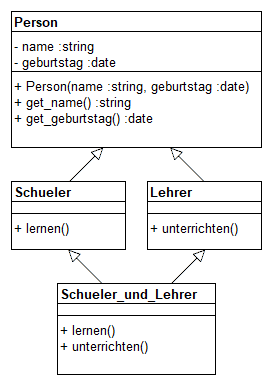
\includegraphics[scale=0.75]{vererbung/mehrfach/diamond/beispiele/schueler_lehrer/schueler_lehrer.png}
					\end{figure}
					
			\paragraph{Java-Lösung}\mbox{}\\
				In Java kann das Diamond-Problem nicht auftreten, da es keine Mehrfachimplementierungsvererbung gibt.
			
	\subsection{Abstrakte Klassen}
		Eine abstrakte Klasse ist eine Klasse, von der keine Objekte erzeugt werden können. Das ist natürlich nur Sinnvoll,
		wenn von so einer Klasse geerbt wird, damit von der Unterklasse ein Objekt erzeugt werden kann. In Java werden
		abstrakte Klassen mit dem abstract-Schlüsselwort gekennzeichnet. In C++ ist eine Klasse, die eine rein virtuelle
		Methode (virtual method() = 0) enthält, automatisch abstrakt.
		
		{\bfseries Java:}
			\UseRawInputEncoding{\lstinputlisting[language={Java}]{vererbung/abstrakt/abstrakt.java}}\inputencoding{utf8}
		
		{\bfseries C++:}
			\UseRawInputEncoding{\lstinputlisting[language={Java}]{vererbung/abstrakt/abstrakt.hpp}}\inputencoding{utf8}
			
			Folgender Code wäre nicht zulässig, da kein Objekt einer abstrakten Klasse erzeugt werden darf.
			\UseRawInputEncoding{\lstinputlisting[language={Java}]{vererbung/abstrakt/abstrakt.use.cpp}}\inputencoding{utf8}
			
			Es muss zuerst von der abstrakten Klasse geerbt werden, um von abgeleiteten Klassen Objekte zu erzeugen. Die rein
			virtuelle Methode muss von der abgeleiteten Klasse implementiert werden, sonst ist auch die abgeleitete Klasse
			abstrakt.
			\UseRawInputEncoding{\lstinputlisting[language={Java}]{vererbung/abstrakt/abstrakt_child.use.cpp}}\inputencoding{utf8}
	
	\subsection{Endgültige Klassen}
		Endgültige Klassen sind Klassen von denen nicht geerbt werden kann.
		\UseRawInputEncoding{\lstinputlisting[language={Java}]{vererbung/endgueltig/endgueltig.hpp}}\inputencoding{utf8}
